\documentclass[]{scrartcl}

\usepackage{amsmath,amssymb}
\usepackage{graphicx}

%opening
\title{Optimal design of experiment}
\author{Oliwer Sliczniuk}

\begin{document}

\maketitle

\begin{abstract}
Notes about the optimal design of an experiment
\end{abstract}

\section{What information do we have?}

\begin{itemize}
	\item Process model: $\dot{x}=f(t,x,p)$
	\item Measurement equation: $\dot{y}=g(x)$
	\item Likelihood function with respect to the dataset
	\item Parameter estimation
	\item Sensitivity equations: $\dot{S} = J_x \dot{x} + J_p$
\end{itemize}

\section{Maximum likelihood}
Let $y^s$ be the vector of all experimental results (random vector) to be used to estimate $p$, and $y^m(p)$. The vector of the corresponding quantities computed by the model $\dot{x}=f(t,x,p)$. For a parallel model, the parameters of which are to be estimated from measurements of an output vector $\dot{y}=g(x)$. We shall call any
oplimizer of $j$, i.e. any $\hat{p}$ that corresponds to an optimal value of the cost function $j$, an estimate of $p$ in the sense of $j$.

The vector $\hat{p}_{ml}$ will be a maximum-likelihood estimate if it maximizes the cost function

\begin{equation}
	j_{ml} = \pi_y (y^s|p) 
\end{equation}

If $p$ were fixed, $\pi_y(y^s|p)$ would be the probability density of the random vector $y^s$ being generated by a model with parameters $p$. Here, to the contrary, $y^s$ is fixed and corresponds to the observations. Considered as a function of $p$, $\pi_y(y^s|p)$ is then called the likelihood of $y^s$. The maximum-likelihood method looks for the value of the parameter vector $p$ that gives the highest likelihood to the observed data. In practice, it is often easier to look for $\hat{p}_{ml}$ by maximizing the log-likelihood function which yields the same estimate since the logarithm function is monotonically increasing.

\begin{equation}
	j_{ml} = \ln ( \pi_y (y^s|p) )
\end{equation}

Assume that the observed outputs satisfy 

\begin{equation}
	y(t_i) = y^m(t_i, p^*) + \epsilon_i, \qquad i=1,...,n_t
\end{equation}

where the vector $y^m(t_i. p^*)$ is the output of a deterministic model, $p^*$ is the true value of the parameter vector and $\epsilon_i$ belongs to a sequence of independent random variables with probability density $\pi_{\epsilon}(\epsilon_i)$. Since the $\epsilon_i$ are independent

\begin{equation}
	\pi_{\epsilon}(\epsilon_1, \epsilon_2, ..., \epsilon_{n_t}) = \prod_{i=1}^{n_t} \pi_{\epsilon_i}(\epsilon_i)
\end{equation}

Consider the output error

\begin{equation}
	e^y(t_i, p) = y(t_i) - y^m(t_i, p)
\end{equation}

For the true value of the parameters, it satisfies $e^y(t_i, p^*)=\epsilon_i$. and, since $y^m$ is deterministic, $\pi_{y_i} (y^s(t_i)|p) = \pi_{\epsilon_i} (e^y(t_i)|p)$. The likelihood of the $n_t$ observations can therefore be written as

\begin{equation}
	 \pi_y (y^s|p) = \prod_{i=1}^{n_t} \pi_{\epsilon_i}(e^y(t_i,p)) =  \prod_{i=1}^{n_t} \pi_{\epsilon_i}(y(t_i) - y^m(t_i, p))
\end{equation}

If the noise is assumed to follow the normal distribution:

\begin{equation}
	\pi_y (y^s|p) = \prod_{i=1}^{n_t} \frac{1}{ \sqrt{2\pi\sigma_i^2} } \exp \left( -\frac{1}{2} \left( \frac{y(t_i) - y^m(t_i, p)}{\sigma_i} \right) \right)
\end{equation}

The associated log-likelihood can be written as

\begin{equation}
	\ln (\pi_y (y^s|p)) = (\text{term independent of p}) - \frac{1}{2} \sum_{i=1}^{n_t}  \left( \frac{y(t_i) - y^m(t_i, p)}{\sigma_{ij}^2} \right)
\end{equation}

Its gradient is thus

\begin{equation}
	\frac{\partial}{\partial p} \ln (\pi_y (y^s|p)) =  \frac{1}{2} \sum_{i=1}^{n_t}  \left( \frac{y(t_i) - y^m(t_i, p)}{\sigma_{ij}^2} \frac{\partial y^m(t_i, p)}{\partial p} \right)
\end{equation}

\section{Fisher information}

The Fisher information is a way of measuring the amount of information that an observable random variable carries about an unknown parameter of a distribution that models the random variable. The Fisher information matrix is used to calculate the covariance matrices associated with maximum-likelihood estimates.

The Fisher information matrix can be calculated as

\begin{align}
	F(p) &= \mathop{\mathbb{E}}_{y^s|p} \left[ \frac{\partial \ln (\pi_y (y^s|p))}{\partial p} \frac{\partial \ln (\pi_y (y^s|p))}{\partial p}^T \right] \\
	&= \mathop{\mathbb{E}}_{y^s|p} \left[ \sum_{k=1}^{n_t} \left( \frac{y(t_k) - y^m(t_k, p)}{\sigma_{t_k}^2} \frac{\partial y^m(t_k, p)}{\partial p} \right) \times  \sum_{i=1}^{n_t} \left( \frac{y(t_i) - y^m(t_i, p)}{\sigma_{t_i}^2} \frac{\partial y^m(t_i, p)}{\partial p^T} \right) \right]
\end{align}

Since

\begin{equation}
	\mathop{\mathbb{E}}_{y^s|p} \left[ \left( y(t_i) - y^m(t_k, p) \right) \left( y(t_i) - y^m(t_i, p) \right) \right] = \sigma_{t_i}^2 \delta_{ik}
\end{equation}

one gets

\begin{equation}
	F(p) = \sum_{i=1}^{n_t} \left( \frac{1}{\sigma_{t_i}^2} \frac{\partial y^m(t_i, p)}{\partial p} \frac{\partial y^m(t_i, p)}{\partial p^T} \right)
\end{equation}

\section{Cramer-Rao inequality}

Let $\hat{p}$ be an (absolutely) unbiased estimator $p^*$, i.e. such that which amounts to saying that if it were possible to replicate the same experiment and
estimate $\hat{p}$ an infinite number of times, the mean of the estimates would coincide with the true value. Let $P$ be the covariance matrix of this estimator. Since $\hat{p}$ is unbiased, $P$ can be written as

\begin{equation}
	P = \mathop{\mathbb{E}}_{y^s|p^*} \left[ \left( \hat{p}(y^s) - p^* \right) \left( \hat{p}(y^s) - p^* \right)^T \right]
\end{equation}

which quantifies how the estimates are spread around the true value $p^*$. One would like the estimates to be as concentrated as possible around this true value, of course. An estimator $\hat{p}_1$ with covariance matrix $P_1$ is said to be more efficient than an estimator $\hat{p}_2$ with covariance matrix $P_2$ if $P_1 < P_2$, that is if $P_2 - P_1$ is positive-definite (i.e.if all the eigenvalues of $P_2-P_1$ arc strictly positive). Since estimators with high efficiency are desirable, a natural request is to make P as small as possible. The Cramer-Rao inequality provides a lower bound to what can be achieved.

Under the hypotheses that:

\begin{itemize}
	\item the set of all data vectors $y^s$ with $\pi_y(y^s|p) > 0$ does not depend on $p$
	\item $\frac{\partial \pi_y(y^s|p)}{\partial p_i}~\left(i=1,2,...,n_p\right)$ is absolutely integrable
	\item $\mathop{\mathbb{E}}_{y^s|p} \left[ \frac{\partial \ln (\pi_y (y^s|p))}{\partial p} \frac{\partial \ln (\pi_y (y^s|p))}{\partial p^T} \right]$ exists and is invertible
\end{itemize}

the covariance of any absolutely unbiased estimator satisfies

\begin{equation}
	P \geq F^{-1}(p^*)
\end{equation}

In other words, the precision to which we can estimate $p$ is fundamentally limited by the Fisher information of the likelihood function.

\section{Experiment design}

The experimental procedure for the collection of the numerical data to be used to estimate the parameters of a given model depends on qualitative choices made at various steps of the modelling. In particular, the tools presented in the previous chapters allow one to choose: 

\begin{itemize}
	\item a set of model structures to be considered
	\item location of sensors and actuators to guarantee identifiability (and distinguishably if several rival structures exist)
	\item an estimator and a characterization of parameter uncertainly
\end{itemize}

Once these choices have been made, the experimenter still has some freedom to specify the quantitative experimental conditions (such as temperature, pressure, sampling times, shape of inputs, etc.). Experiment design aims at determining experimental conditions adapted to the final purpose of the modelling. It is a crucial step, for a badly designed experiment may ruin any attempt at analysing the data collected from the system.

Assume that the i'th scalar observation can be written as $y(\xi_i)$, where the $n_\xi$-dimensional vector $\xi_i$ (the i'th support point) describes the experimental conditions (e.g., measurement time, shape of input...) under which the i'th observation is to be collected. When $n_t$ such observations are taken, the concatenation of the vectors $\xi_i$'s yields the $\Xi = (\xi_1, \xi_2,..., \xi_{n_t})$, which characterizes all experimental conditions to be optimized. To make experiment design realistic, it is necessary to take a number of constraints into account, e.g. on the duration of the experiments, the energy or amplitude of the inputs, the minimum time between samples. Let $\bar{\Xi}$ be the set of all feasible values for $\Xi$. 

The definition of a cost function $j$ then permits optimal experiment design to be cast as a constrained optimization problem, where the optimal experiment $\Xi^*$ is defined by

\begin{equation}
	\Xi^* = \arg~\underset{\Xi \in \bar{\Xi}}{\text{opt}}~j\left(\Xi\right)
\end{equation}

Evaluation of the cost function $j$ must be simple enough to allow easy optimization. For that reason, classical oplimality criteria correspond to a scalar function of the Fisher information matrix $F(p,\Xi)$

\begin{equation}
	j(\Xi) = \phi\left[ F(p, \Xi) \right]
\end{equation}

Under the hypotheses mentioned above, the distribution of the maximum likelihood estimator is asymptotically Gaussian $\mathop{\mathbb{N}} (p^*, F^{-1}([^*, \Xi])) $ when the number of measurements tends to infinity. Minimizing $j(\Xi)$ then amounts to minimizing a scalar easure of the asymptotic covariance matrix of the parameters.

A rather general class of optimality criteria employs the following family of cost functions

\begin{align}
	\phi_k(F) &= \left[\frac{1}{n_p} \text{trace}\left( QF^{-1}Q^T \right)^k \right]^{1/k} \quad &if \det F \neq 0 \nonumber \\
	\phi_k(F) &= \infty \quad &if \det F = 0
\end{align}

where $Q$ is a weighting matrix. The special case $k = 1$ corresponds to the L-optimality cost function,

\begin{equation}
	j_L(\Xi) = \text{trace} \left[ Q^TQF^{-1}(p,\Xi) \right]
\end{equation}

and choosing $Q = \textbf{I}_{n_p}$ then corresponds to the A-optimality cost function. An A-optimal experiment minimizes the sum of the squares of the lengths or the axes of asymptotic confidence ellipsoids. Choosing $Q$ diagonal, with $[Q]_{ii} = 1/p_i$ corresponds to C-optimality, which is connected with the relative precision of estimates. Taking Q to be a row vector leads to c-optimality. Taking $Q = \textbf{I}_{n_p}$ and $k = \infty$ corresponds to E-optimality; E-optimal design maximizes the smallest eigenvalues of the Fisher information matrix and thus minimizes the length of the largest axis of the asymptotic confidence ellipsoids. The most widely used optimality criterion has $k = 0$, $Q = \textbf{I}_{n_p}$ , requiring minimization of $\det F^{-1}(p, \Xi)$, or, equivalently, maximization of

\begin{equation}
	j_D(\Xi) = \det F(p, \Xi)
\end{equation}

A D-optimal experiment minimizes the volume of the asymptotic confidence ellipsoids for the parameters.

\begin{figure}[h]
	\centering
	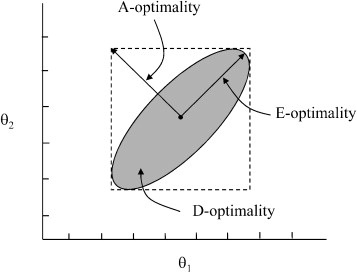
\includegraphics[width=8cm]{DOE_conditions.jpg}
\end{figure}


\end{document}

































